\documentclass[]{article}
\usepackage{lmodern}
\usepackage{amssymb,amsmath}
\usepackage{ifxetex,ifluatex}
\usepackage{fixltx2e} % provides \textsubscript
\ifnum 0\ifxetex 1\fi\ifluatex 1\fi=0 % if pdftex
  \usepackage[T1]{fontenc}
  \usepackage[utf8]{inputenc}
\else % if luatex or xelatex
  \ifxetex
    \usepackage{mathspec}
  \else
    \usepackage{fontspec}
  \fi
  \defaultfontfeatures{Ligatures=TeX,Scale=MatchLowercase}
  \newcommand{\euro}{€}
\fi
% use upquote if available, for straight quotes in verbatim environments
\IfFileExists{upquote.sty}{\usepackage{upquote}}{}
% use microtype if available
\IfFileExists{microtype.sty}{%
\usepackage{microtype}
\UseMicrotypeSet[protrusion]{basicmath} % disable protrusion for tt fonts
}{}
\usepackage[margin=1in]{geometry}
\usepackage{hyperref}
\PassOptionsToPackage{usenames,dvipsnames}{color} % color is loaded by hyperref
\hypersetup{unicode=true,
            pdftitle={wCorr Arguments},
            pdfauthor={Paul Bailey},
            pdfborder={0 0 0},
            breaklinks=true}
\urlstyle{same}  % don't use monospace font for urls
\usepackage{color}
\usepackage{fancyvrb}
\newcommand{\VerbBar}{|}
\newcommand{\VERB}{\Verb[commandchars=\\\{\}]}
\DefineVerbatimEnvironment{Highlighting}{Verbatim}{commandchars=\\\{\}}
% Add ',fontsize=\small' for more characters per line
\usepackage{framed}
\definecolor{shadecolor}{RGB}{248,248,248}
\newenvironment{Shaded}{\begin{snugshade}}{\end{snugshade}}
\newcommand{\KeywordTok}[1]{\textcolor[rgb]{0.13,0.29,0.53}{\textbf{{#1}}}}
\newcommand{\DataTypeTok}[1]{\textcolor[rgb]{0.13,0.29,0.53}{{#1}}}
\newcommand{\DecValTok}[1]{\textcolor[rgb]{0.00,0.00,0.81}{{#1}}}
\newcommand{\BaseNTok}[1]{\textcolor[rgb]{0.00,0.00,0.81}{{#1}}}
\newcommand{\FloatTok}[1]{\textcolor[rgb]{0.00,0.00,0.81}{{#1}}}
\newcommand{\ConstantTok}[1]{\textcolor[rgb]{0.00,0.00,0.00}{{#1}}}
\newcommand{\CharTok}[1]{\textcolor[rgb]{0.31,0.60,0.02}{{#1}}}
\newcommand{\SpecialCharTok}[1]{\textcolor[rgb]{0.00,0.00,0.00}{{#1}}}
\newcommand{\StringTok}[1]{\textcolor[rgb]{0.31,0.60,0.02}{{#1}}}
\newcommand{\VerbatimStringTok}[1]{\textcolor[rgb]{0.31,0.60,0.02}{{#1}}}
\newcommand{\SpecialStringTok}[1]{\textcolor[rgb]{0.31,0.60,0.02}{{#1}}}
\newcommand{\ImportTok}[1]{{#1}}
\newcommand{\CommentTok}[1]{\textcolor[rgb]{0.56,0.35,0.01}{\textit{{#1}}}}
\newcommand{\DocumentationTok}[1]{\textcolor[rgb]{0.56,0.35,0.01}{\textbf{\textit{{#1}}}}}
\newcommand{\AnnotationTok}[1]{\textcolor[rgb]{0.56,0.35,0.01}{\textbf{\textit{{#1}}}}}
\newcommand{\CommentVarTok}[1]{\textcolor[rgb]{0.56,0.35,0.01}{\textbf{\textit{{#1}}}}}
\newcommand{\OtherTok}[1]{\textcolor[rgb]{0.56,0.35,0.01}{{#1}}}
\newcommand{\FunctionTok}[1]{\textcolor[rgb]{0.00,0.00,0.00}{{#1}}}
\newcommand{\VariableTok}[1]{\textcolor[rgb]{0.00,0.00,0.00}{{#1}}}
\newcommand{\ControlFlowTok}[1]{\textcolor[rgb]{0.13,0.29,0.53}{\textbf{{#1}}}}
\newcommand{\OperatorTok}[1]{\textcolor[rgb]{0.81,0.36,0.00}{\textbf{{#1}}}}
\newcommand{\BuiltInTok}[1]{{#1}}
\newcommand{\ExtensionTok}[1]{{#1}}
\newcommand{\PreprocessorTok}[1]{\textcolor[rgb]{0.56,0.35,0.01}{\textit{{#1}}}}
\newcommand{\AttributeTok}[1]{\textcolor[rgb]{0.77,0.63,0.00}{{#1}}}
\newcommand{\RegionMarkerTok}[1]{{#1}}
\newcommand{\InformationTok}[1]{\textcolor[rgb]{0.56,0.35,0.01}{\textbf{\textit{{#1}}}}}
\newcommand{\WarningTok}[1]{\textcolor[rgb]{0.56,0.35,0.01}{\textbf{\textit{{#1}}}}}
\newcommand{\AlertTok}[1]{\textcolor[rgb]{0.94,0.16,0.16}{{#1}}}
\newcommand{\ErrorTok}[1]{\textcolor[rgb]{0.64,0.00,0.00}{\textbf{{#1}}}}
\newcommand{\NormalTok}[1]{{#1}}
\usepackage{longtable,booktabs}
\usepackage{graphicx,grffile}
\makeatletter
\def\maxwidth{\ifdim\Gin@nat@width>\linewidth\linewidth\else\Gin@nat@width\fi}
\def\maxheight{\ifdim\Gin@nat@height>\textheight\textheight\else\Gin@nat@height\fi}
\makeatother
% Scale images if necessary, so that they will not overflow the page
% margins by default, and it is still possible to overwrite the defaults
% using explicit options in \includegraphics[width, height, ...]{}
\setkeys{Gin}{width=\maxwidth,height=\maxheight,keepaspectratio}
\setlength{\parindent}{0pt}
\setlength{\parskip}{6pt plus 2pt minus 1pt}
\setlength{\emergencystretch}{3em}  % prevent overfull lines
\providecommand{\tightlist}{%
  \setlength{\itemsep}{0pt}\setlength{\parskip}{0pt}}
\setcounter{secnumdepth}{0}

%%% Use protect on footnotes to avoid problems with footnotes in titles
\let\rmarkdownfootnote\footnote%
\def\footnote{\protect\rmarkdownfootnote}

%%% Change title format to be more compact
\usepackage{titling}

% Create subtitle command for use in maketitle
\newcommand{\subtitle}[1]{
  \posttitle{
    \begin{center}\large#1\end{center}
    }
}

\setlength{\droptitle}{-2em}
  \title{wCorr Arguments}
  \pretitle{\vspace{\droptitle}\centering\huge}
  \posttitle{\par}
  \author{Paul Bailey}
  \preauthor{\centering\large\emph}
  \postauthor{\par}
  \predate{\centering\large\emph}
  \postdate{\par}
  \date{2016-03-04}



% Redefines (sub)paragraphs to behave more like sections
\ifx\paragraph\undefined\else
\let\oldparagraph\paragraph
\renewcommand{\paragraph}[1]{\oldparagraph{#1}\mbox{}}
\fi
\ifx\subparagraph\undefined\else
\let\oldsubparagraph\subparagraph
\renewcommand{\subparagraph}[1]{\oldsubparagraph{#1}\mbox{}}
\fi

\begin{document}
\maketitle

This vignette explores two Boolean switches in the wCorr package. First,
the \texttt{ML} switch allows for either a non-MLE (but consistent)
esitimate of the nusiance parameters that define the binning process to
be used (\texttt{ML=FALSE}) or for the nusiance parameters to be
estimated using the MLE (\texttt{ML=TRUE}). Second the \texttt{fast}
argument gives the option to use a pure R implementation
(\texttt{fast=FALSE}) or an implementation that relies on the
\texttt{Rcpp} and \texttt{RcppArmadillo} packages (\texttt{fast=TRUE}).

Numerical simulations in this vignette show that differences in the
results are essentially unaffected by either of these switches.

The \emph{wCorr Formulas} vignette describes the statistical properties
of the correlation estimators in the package and has a more complete
derivation of the likelihood functions.

\section{\texorpdfstring{The \texttt{ML}
switch}{The ML switch}}\label{the-ml-switch}

The correlation coefficients between two vectors of random variables
that are jointly bivariate normal--call the vectors \textbf{\emph{X}}
and \textbf{\emph{Y}}.

\[\begin{pmatrix} X \\ Y \end{pmatrix} \sim N \left[ \begin{pmatrix} \mu_x \\ \mu_y \end{pmatrix}, \boldsymbol{\Sigma} \right] \]

where \(N(\mathbf{A},\boldsymbol{\Sigma})\) is the bivariate normal
distribution with mean \textbf{\emph{A}} and covariance
\(\boldsymbol{\Sigma}\).

\subsection{Polyserial computation}\label{polyserial-computation}

the likelihood function for an individual observation of the polyserial
is\footnote{See the ``wCorr Formulas'' vignette for a more complete
  description and motivation for the polyserial correlations's
  likelihood function.}

\[\mathrm{Pr}\left( \rho=r, \boldsymbol{\theta} ; Z=z_i, M=m_i \right) = \phi(z_i) \left[ \Phi\left( \frac{\theta_{m_i+2} - r \cdot z_i}{\sqrt{1-r^2}} \right) - \Phi \left( \frac{\theta_{m_i+1} - r \cdot z_i}{\sqrt{1-r^2}} \right) \right]\]

where \(\rho\) is the correlation between \textbf{\emph{X}} and
\textbf{\emph{Y}}, \textbf{\emph{Z}} is the normalized version of
\textbf{\emph{X}}, and \textbf{\emph{M}} is a discretized version of
\textbf{\emph{Y}}, using \(\boldsymbol{\theta}\) as cut points as
described in the ``\emph{Corr Formulas} vignette.

The log-likelihood is then

\[\ell(\rho, \boldsymbol{\theta};z,m) = \sum_i w_i \ln\left[ \mathrm{Pr}\left( \rho=r, \boldsymbol{\theta} ; Z=z_i, M=m_i \right) \right]\]

The derivatives of \(\ell\) can be computed but are not readily computed
and so when the \texttt{ML} argumet is set to \texttt{FALSE} (the
default) a one dimensional optimization of \(\rho\) is calculated using
\texttt{stats::optimize}. When the \texttt{ML} argument is set to
\texttt{TRUE} a multi-dimensional optimization is done for \(\rho\) and
\(\boldsymbol{\theta}\) using \texttt{minqa::bobyqa}.

\subsection{Polychoric computation}\label{polychoric-computation}

the likelihood function for the polychoric is\footnote{See the ``wCorr
  Formulas'' vignette for a more complete description and motivation for
  the polychoric correlations's likelihood function.}

\[\mathrm{Pr}\left( \rho=r, \boldsymbol{\theta}, \boldsymbol{\theta}' ; P=p_i, M=m_i \right) = \int_{\theta_{p_i+1}'}^{\theta_{p_i+2}'} dx \int_{\theta_{m_i+1}}^{\theta_{m_i+2}} \mkern-40mu dy f(x,y|\rho=r)\]

where \(f(x,y|r)\) is the noramlzied bivariate normal distribution with
correlation \(\rho\).

The log-likelihood is then
\[\ell(\rho, \boldsymbol{\theta}, \boldsymbol{\theta}' ;p,m) = \sum_i w_i \ln\left[\mathrm{Pr}\left( \rho=r, \boldsymbol{\theta}, \boldsymbol{\theta}' ; P=p_i, M=m_i \right) \right] \]

The derivatives of \(\ell\) can be computed but are not readily computed
and so when the \texttt{ML} argumet is set to \texttt{FALSE} (the
default) a one dimensional optimization of \(\rho\) is calculated using
\texttt{stats::optimize}. When the \texttt{ML} argument is set to
\texttt{TRUE} a multi-dimensional optimization is done for \(\rho\),
\(\boldsymbol{\theta}\), and \(\boldsymbol{\theta}'\) using
\texttt{minqa::bobyqa}.

\section{General setup for the unweighted
case}\label{general-setup-for-the-unweighted-case}

A simulation is run several times. For each itteration, the following
procedure is used:

\begin{itemize}
\tightlist
\item
  select the number of observations (\(n\))
\item
  select a true correlation coefficient \(\rho\)
\item
  generate \textbf{\emph{X}} and \textbf{\emph{Y}} to be bivariate
  normally distributed using a pseudo-Random Number Generator (RNG)
\item
  using a pseudo-RNG, select the the number of bins for
  \textbf{\emph{M}} and \textbf{\emph{P}} (\(t\) and \(t'\))
  independantly from the set \{2, 3, 4, 5\}
\item
  select the bin boundaries for \textbf{\emph{M}} and \textbf{\emph{P}}
  (\(\boldsymbol{\theta}\) and \(\boldsymbol{\theta}'\)) by sorting the
  results of \(t\) and \(t'\) draws, respectively, from a normal
  distribution using a pseudo-RNG
\item
  confirm that at least 2 levels of each of \textbf{\emph{M}} and
  \textbf{\emph{P}} are occupied (if not, retrun to generating
  \textbf{\emph{X}} and \textbf{\emph{Y}})
\item
  calculate and record relevant statistics
\end{itemize}

when the exact method of selecting a parameter (such as \(n\)) is not
noted in the above description it is described as part of each
simulation.

\section{ML switch}\label{ml-switch}

A simulation was done at each level of the cartesian product of
\(\mathtt{ML} \in \{\mathtt{TRUE}, \mathtt{FALSE} \}\),
\(\rho \in \left( -0.99, -0.95, -0.90, -0.85, ..., 0.95, 0.99 \right)\),
and \(n \in \{10, 100, 1000\}\). For precision, each iteration is run
three times. The compulation is run so that the same values of the
variables are used for \texttt{ML=TRUE} as \texttt{ML=FALSE} and then
the statistics are comared between the two sets of results. where
\(MAD\) is the mean absolute difference and is given by

\[MAD= | r_{ML=TRUE} - r_{ML=FALSE} |  \]

where \(r_{ML=TRUE}\) is the estimated correlation when \texttt{ML=TRUE}
and \(r_{ML=FALSE}\) is the estimated correlation when
\texttt{ML=FALSE}.

This is a plot of the \(MAD\) as a function of the true correlation
coefficnet.

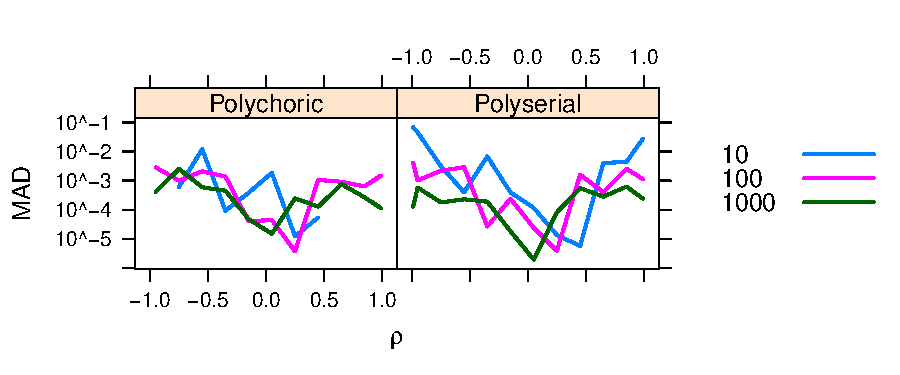
\includegraphics{wCorrArguments_files/figure-latex/unnamed-chunk-1-1.pdf}

This table shows the \(MAD\) by \(n\) and correlation type.

\begin{Shaded}
\begin{Highlighting}[]
\NormalTok{agg <-}\StringTok{ }\KeywordTok{summaryBy}\NormalTok{(absdrho ~}\StringTok{ }\NormalTok{type+n, }\DataTypeTok{data=}\NormalTok{mml, }\DataTypeTok{FUN=}\NormalTok{mean, }\DataTypeTok{na.rm=}\OtherTok{TRUE}\NormalTok{)}
\KeywordTok{colnames}\NormalTok{(agg) <-}\StringTok{ }\KeywordTok{c}\NormalTok{(}\StringTok{"Correlation type"}\NormalTok{, }\StringTok{"n"}\NormalTok{, }\StringTok{"MAD"}\NormalTok{)}
\KeywordTok{kable}\NormalTok{(agg)}
\end{Highlighting}
\end{Shaded}

\begin{longtable}[c]{@{}lrr@{}}
\toprule
Correlation type & n & MAD\tabularnewline
\midrule
\endhead
Polychoric & 10 & 0.0012567\tabularnewline
Polychoric & 100 & 0.0009644\tabularnewline
Polychoric & 1000 & 0.0004658\tabularnewline
Polyserial & 10 & 0.0134924\tabularnewline
Polyserial & 100 & 0.0013627\tabularnewline
Polyserial & 1000 & 0.0002594\tabularnewline
\bottomrule
\end{longtable}

\section{fast switch}\label{fast-switch}

This section looks at the agreement between the pure R implementation of
the optimizations and the \texttt{Rcpp} and \texttt{RcppArmadillo}
impelemntation. The code can compute with either option by setting
\texttt{fast=FALSE} (pure R) or \texttt{fast=TRUE} (Rcpp).

This is the summary of all differences between the \texttt{fast=TRUE}
and \texttt{fast=FALSE\ runs} for the polyserial

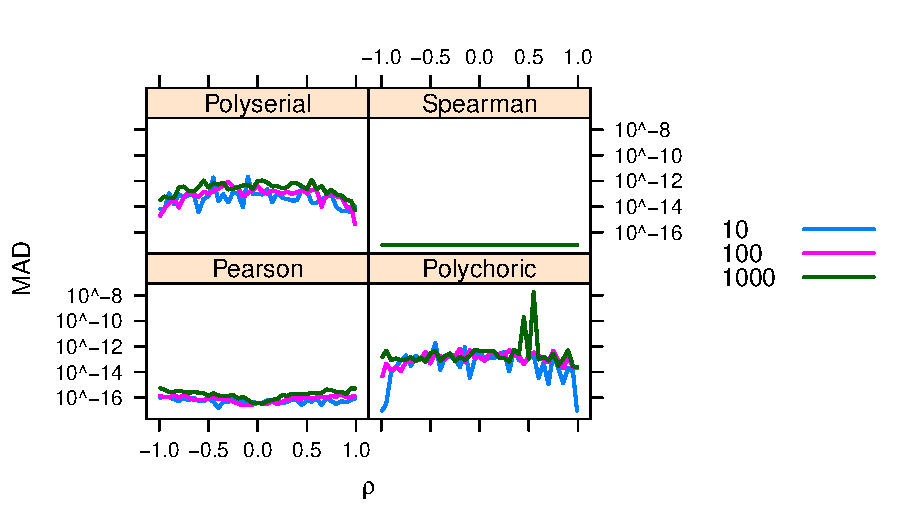
\includegraphics{wCorrArguments_files/figure-latex/unnamed-chunk-3-1.pdf}

This table shows the \(MAD\) by \(n\) and correlation type.

\begin{longtable}[c]{@{}lrr@{}}
\toprule
Correlation type & n & MAD\tabularnewline
\midrule
\endhead
Pearson & 10 & 0\tabularnewline
Pearson & 100 & 0\tabularnewline
Pearson & 1000 & 0\tabularnewline
Polychoric & 10 & 0\tabularnewline
Polychoric & 100 & 0\tabularnewline
Polychoric & 1000 & 0\tabularnewline
Polyserial & 10 & 0\tabularnewline
Polyserial & 100 & 0\tabularnewline
Polyserial & 1000 & 0\tabularnewline
Spearman & 10 & 0\tabularnewline
Spearman & 100 & 0\tabularnewline
Spearman & 1000 & 0\tabularnewline
\bottomrule
\end{longtable}

\section{Implications for speed}\label{implications-for-speed}

A simulation was done at each level of the cartesian product of
\(\mathtt{ML} \in \{\mathtt{TRUE}, \mathtt{FALSE} \}\),
\(\mathtt{fast} \in \{\mathtt{TRUE}, \mathtt{FALSE} \}\),
\(\rho \in \left( -0.99, -0.95, -0.90, -0.85, ..., 0.95, 0.99 \right)\),
and \(n \in \{10^1, 10^{1.25}, 10^{1.5}, ..., 10^7\}\). For precision,
each iteration is run three times. The compulation is run so that the
same values of the variables are used all four levels of \texttt{ML} and
\texttt{fast}. The variety of correlations is chosen so that the results
represent an average of possible values of \(\rho\).

The following plot shows the mean compute time versus \(n\).

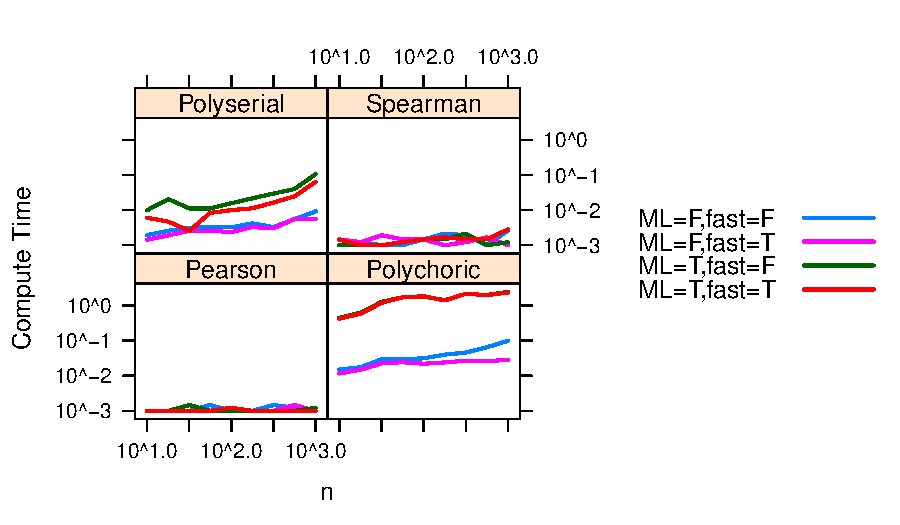
\includegraphics{./tex2pdf.25548/1cd97661318e4d1b89fbc91a222d4823a8a80b5c.pdf}

\end{document}
